A common approach for MIL is to use some form of dissimilarity measure in the classification of new bags. 
For instance-level information, the dissimilarity is measured between the instances in a bag and instances in labelled bags or prototypes. 
Examples are the Harrington distance, and its variants. 
For bag-level information, the dissimilarity is measured between the bag as a whole and labelled bags or prototypes. 
For explicit information, the dissimilarity is calculated based on the instance values.
For implicit information, the instance values are transformed to a single vector (e.g. the median), and a single-instance dissimilarity measure can be used. 
Hybrid versions also exist, see e.g. {\color{green} Chepuliga (2016)}. 

We here introduce two new approaches that has not been studied in the MIL context: 
(1) Divergence-based dissimilarity measures. 
(2) Bag-to-class dissimilarities. 

A divergence function (or simply divergence) is a measure of dissimilarity between two probability distributions.
A divergence does not necessarily fulfil the mathematical requirements of a distance, especially the triangle inequality. 
In the MIL context, the instances of a bag form the basis of a probability distribution estimate, and then a divergence can be applied. \\
\begin{align}
  D(P_{bag}, P_{ref})\, ,
\end{align}
where $P_{bag}$ is the probability distribution of the bag that we want to classify, and $P_{ref}$ is the reference distribution. 
$P_{ref}$ can be any distribution, but would typically be that of labelled bags, classes, or prototype distributions. 

In practice, the distributions must be estimated from the instances of the bag, using the assumption that they are independent observations from a common underlying distribution. 
Commonly used is the EM-algorithm.
Which method to apply for distribution estimation depends on the data, especially the sparsity, previous knowledge, and requirements regarding time consumption. 
We will not go into the details, but simply use the EM-algorithm.
Assuming that the instances are observations from an underlying distribution. 

The bag-to-class dissimilarity has not been used in MIL, although there are obvious advantages:
For one, the computation time decreases when the dissimilarity is calculated only between a bag and the classes, compared to pairwise dissimilarities between a bag and all labelled bags or prototypes. 
A class can be seen as a prototype, and in that case, bag-to-class will be the minimum number of prototypes. 
We propose a dissimilarity measure fro bag-to-class comparison, based on the divergence between two probability distributions. 
We will also shortly discuss divergence for bag-to-bag comparison. 
A bag-to-class approach can be used without a divergence. 

A huge variation among divergences exists.
Popular functions are the Kullback-Leibler information (non-symmetric), the KL divergence, the Shannon entropy, and many more. 
Choice of divergence must reflect the problem at hand. 
%For several areas, the original divergence is alteret to fit the problem, e.g. in clustering, where the size of the subcluster can be of great importance. 
See e.g. {\color{green} Mollersen et al} for properties of some common divergences. 

%Let there be two classes, positive and negative. 
%An instance, $x_i$ is a sample from an underlying distribution, $P_{pos}$ or $P_{neg}$. 
%A bag contains instances from a hierarchical distribution
%\begin{align}
%  X_{ij} \sim \pi_j P_+ + (1-\pi) P_- \, ,
%\end{align}
%where $\pi_j$ is a parameter of the class. 
%This means that we can allow both positive and negative instances to appear in both positive and negative bags.
%Ultimately, $P_{bag, pos} \neq P_{bag, neg}$, or else they cannot be distinguished, so we require $\pi_{pos} \neq \pi_{neg}$.
%
%In the standard assumptions, we have
%\begin{align}
%  X_{i, {pos}} \sim \pi_{pos}P_+ + (1-\pi_{pos}) P_- \, ,
%\end{align}
%where $\pi_{pos} > 0$, and
%\begin{align}
%  X_{i,{neg}} \sim P_-
%\end{align}
%This can be relaxed to 
%\begin{align}
%  X_{i,pos} & \sim \pi_{pos}P_+ + (1-\pi_{pos}) P_- \\
%  X_{i,neg} & \sim \pi_{neg}P_+ + (1-\pi_{neg}) P_- \, ,
%\end{align}
%where $\pi_{pos} \sim P_{\pi_{pos}}$ and $\pi_{neg} \sim P_{\pi_{neg}}$, where $P_{\pi_{pos}} \neq P_{\pi_{neg}}$. 
%This corresponds to the top level of Weidmanns hierarchy. 
%
%We assume that $P_+$ and $P_-$ are parametrised distributions, where $\theta_+$ and $\theta_-$ follow distributions on their own. 
%This means that within a bag, $\theta_+$ and $\theta_-$ are constants, but varies between bags. 
%We believe this is a more realistic approach than assuming that all positive instances come from the same distribution. 
%
%Example: \\
%\begin{align}
%  P_+:  \, &\mathcal{N} (\mu_+, \sigma_+^2) \\
%  \mu_+ \sim & \mathcal{N} (\nu_\mu, \tau_\mu^2) \\
%  \sigma_+^2  \sim & \mathcal{N} (\nu_\sigma, \tau_\sigma^2),   
%\end{align}
%where $\nu$ and $\tau$ are constants, and $\mu_+$ and $\sigma_+$ are drawn once for each bag. 
%
%The two class distributions are estimated based on the bag labels. 
The goal is not to distinguish between $P_+$ and $P_-$.
We will get $P_{pos}$ and $P_{neg}$. 
For a new bag, we want to measure $D(P_{bag},P_{pos})$ and/or $D(P_{bag},P_{neg})$.
It is important to notice that $P_{pos}$ is not equal to any $P_{bag, pos}$, but rather a collection of all possible $P_{bag,pos}$s with their probability of occurrence taken in mind.
Therefore, symmetry of the divergence is not a requirement.

Let $\mathcal{X}_{pos>{bag,pos}}$ be the region where $p_{pos}(x)>p_{bag,pos}(x)$. 
Then $\mathcal{X}_{pos>{bag,pos}} \geq \mathcal{X}_{pos \leq {bag,pos}}$, 
meaning that the region where $p_{pos}$ is greater than $p_{p\_ bag}$ is bigger than the opposite. 
This comes from the hierarchical nature of $P_{pos}$, where $\theta_{pos} = [\pi_{pos} \,\,\,\theta_+ \,\,\,\theta_-]$ has a distribution, and $p_{p\_ bag}$ is uniquely defined by the $\theta_{pos}$ sample. 
An illustration
\begin{figure}[!h]
  \centering
  \begin{subfigure}{}
    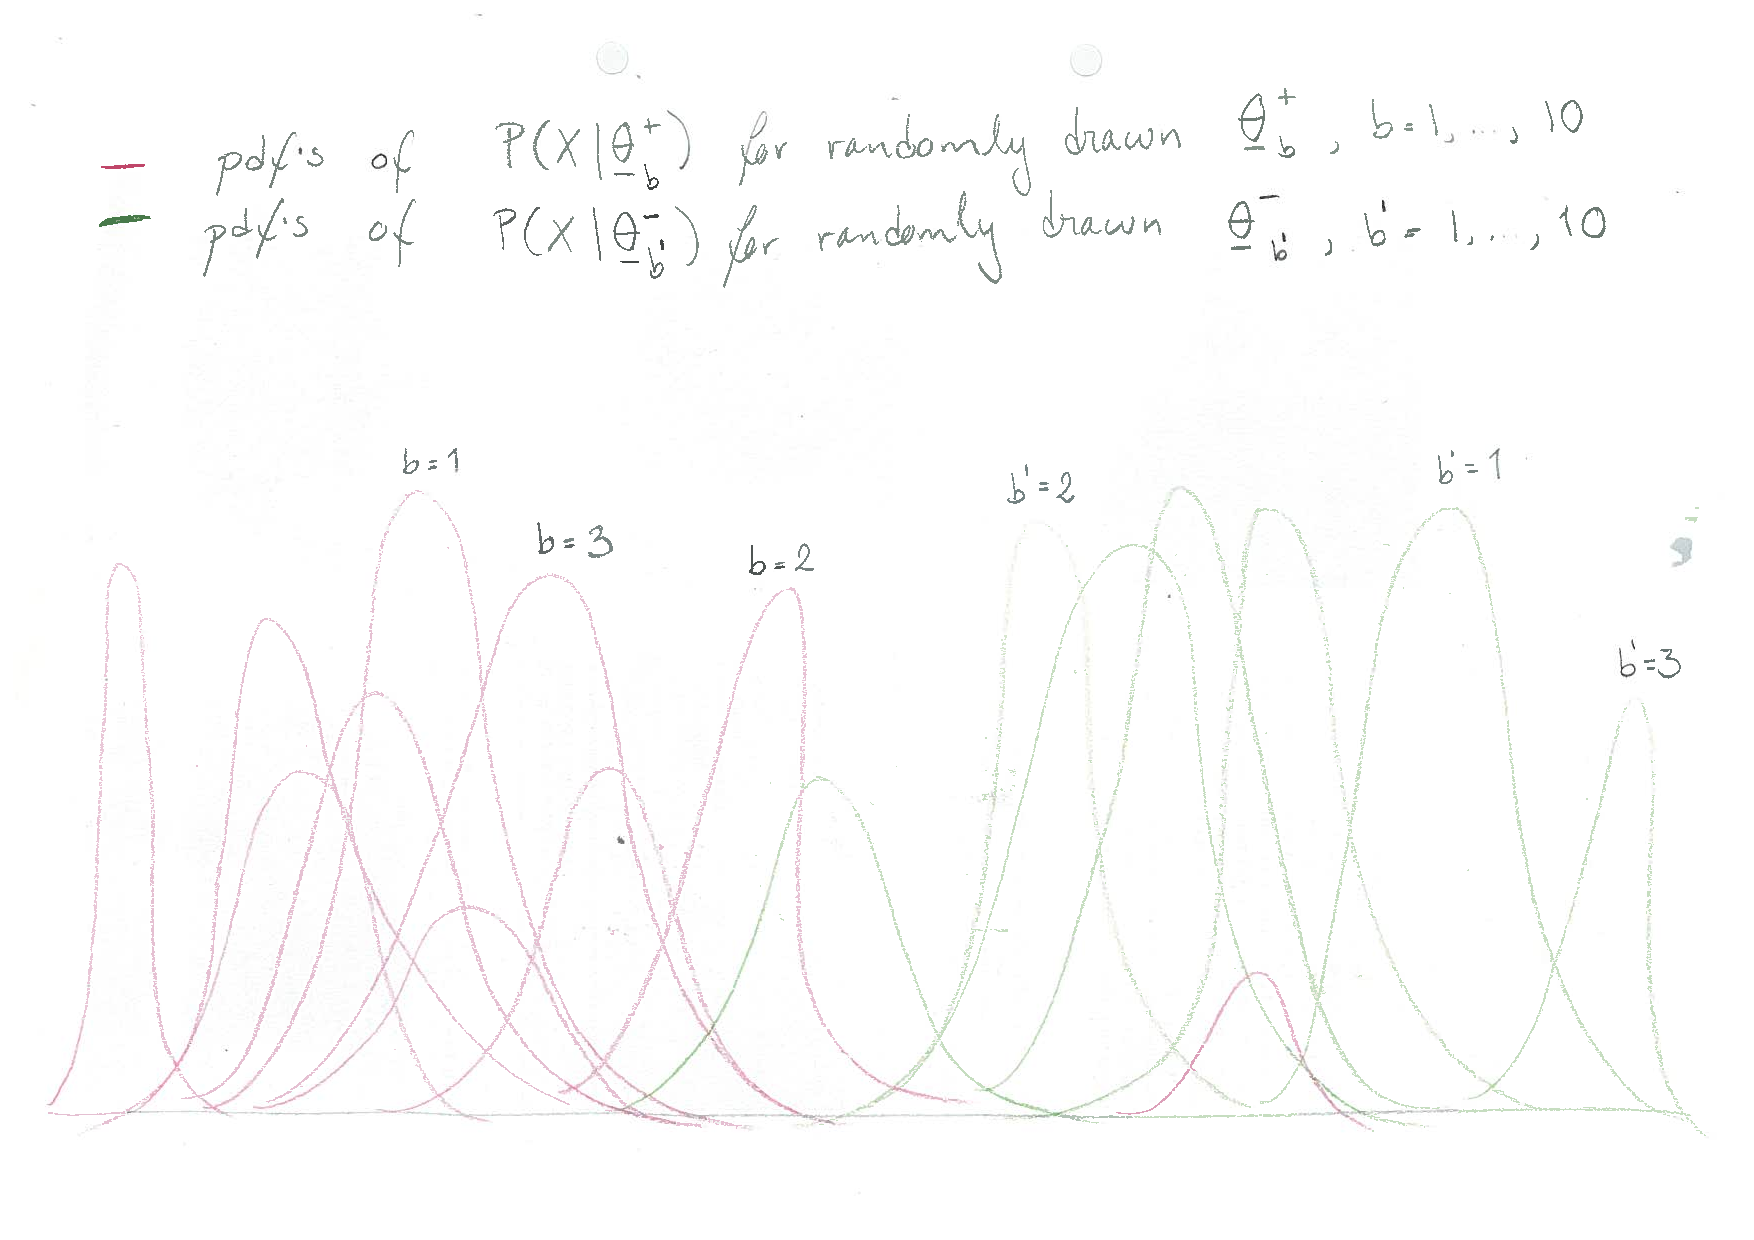
\includegraphics[height = 0.3\textheight]{/Volumes/kam025/Documents/Figures/Divergence_Manuscript/distrs.pdf}
  \end{subfigure}    
  \begin{subfigure}{}
    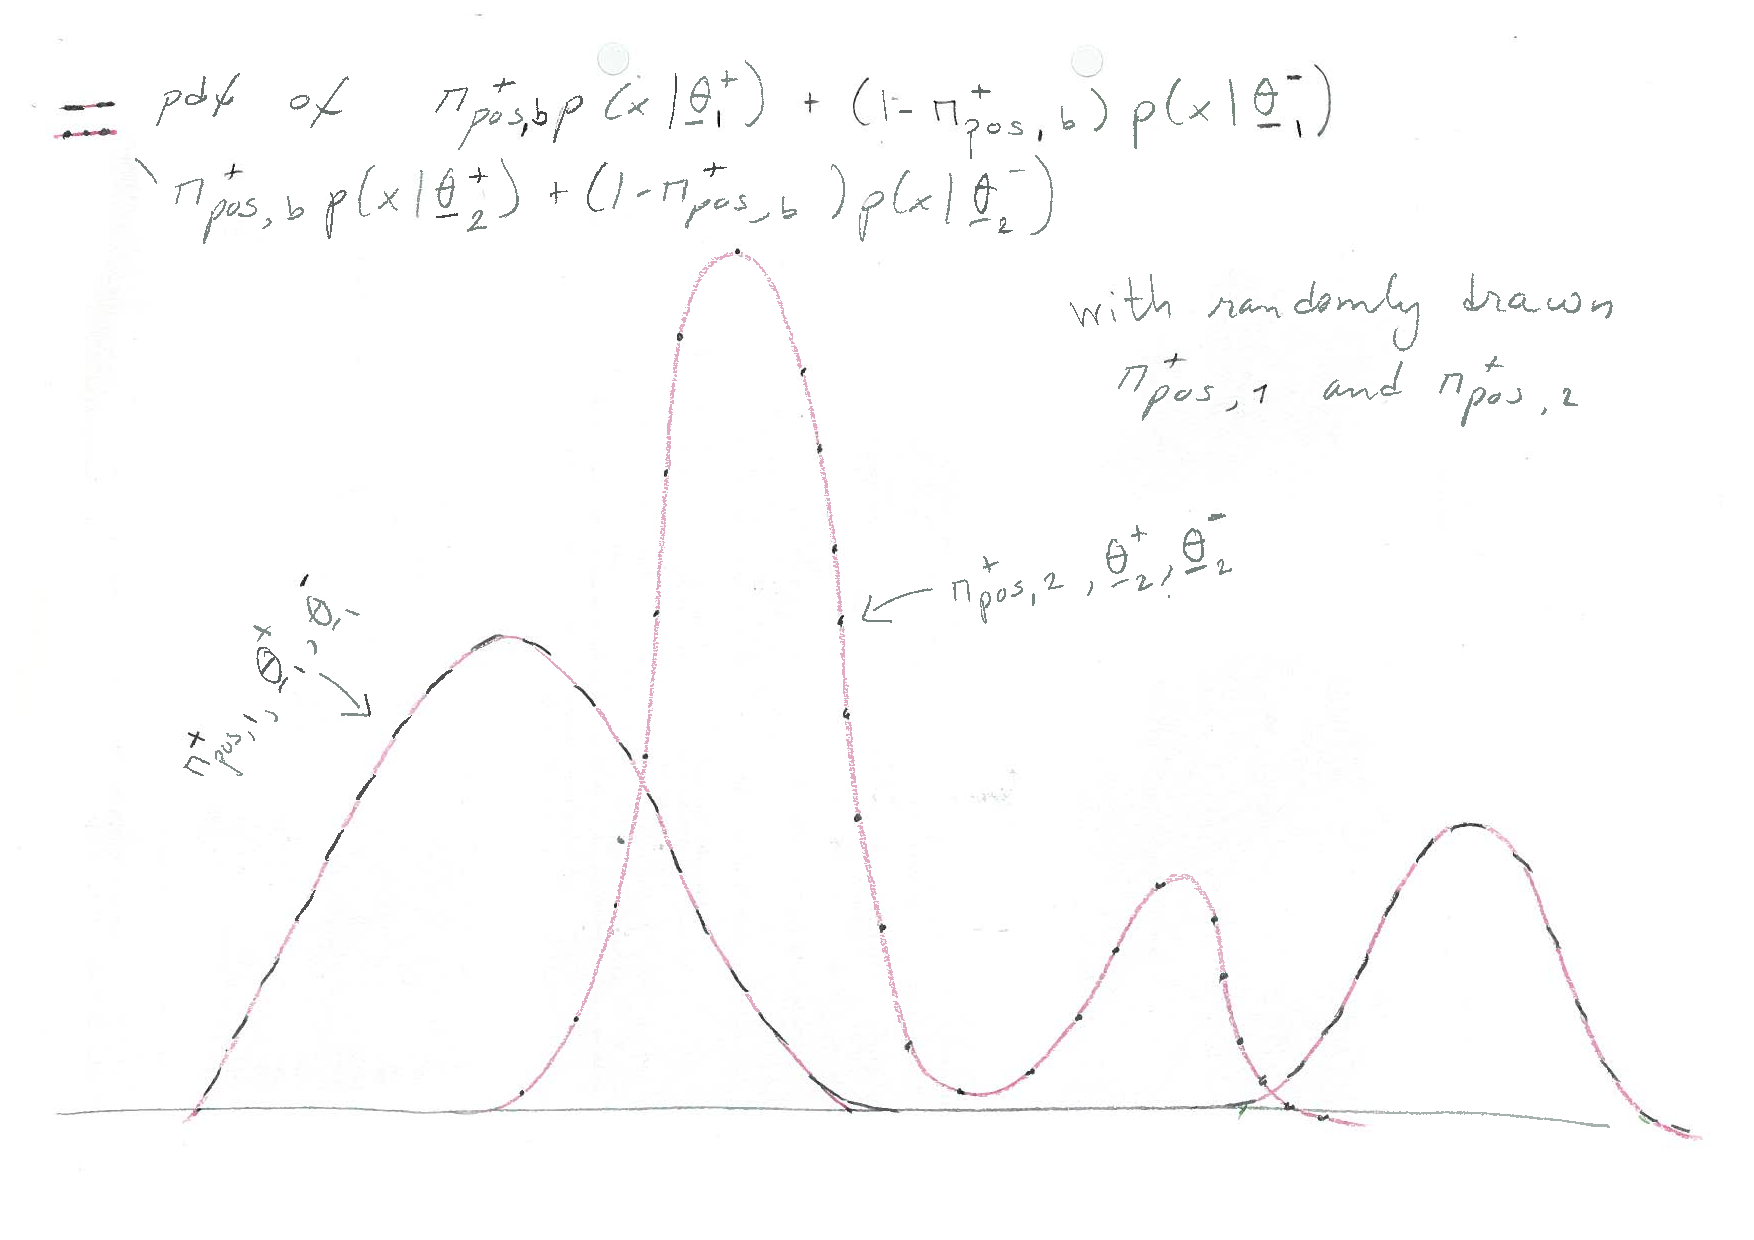
\includegraphics[height = 0.3\textheight]{/Volumes/kam025/Documents/Figures/Divergence_Manuscript/pos.pdf}
  \end{subfigure}
  \begin{subfigure}{}
    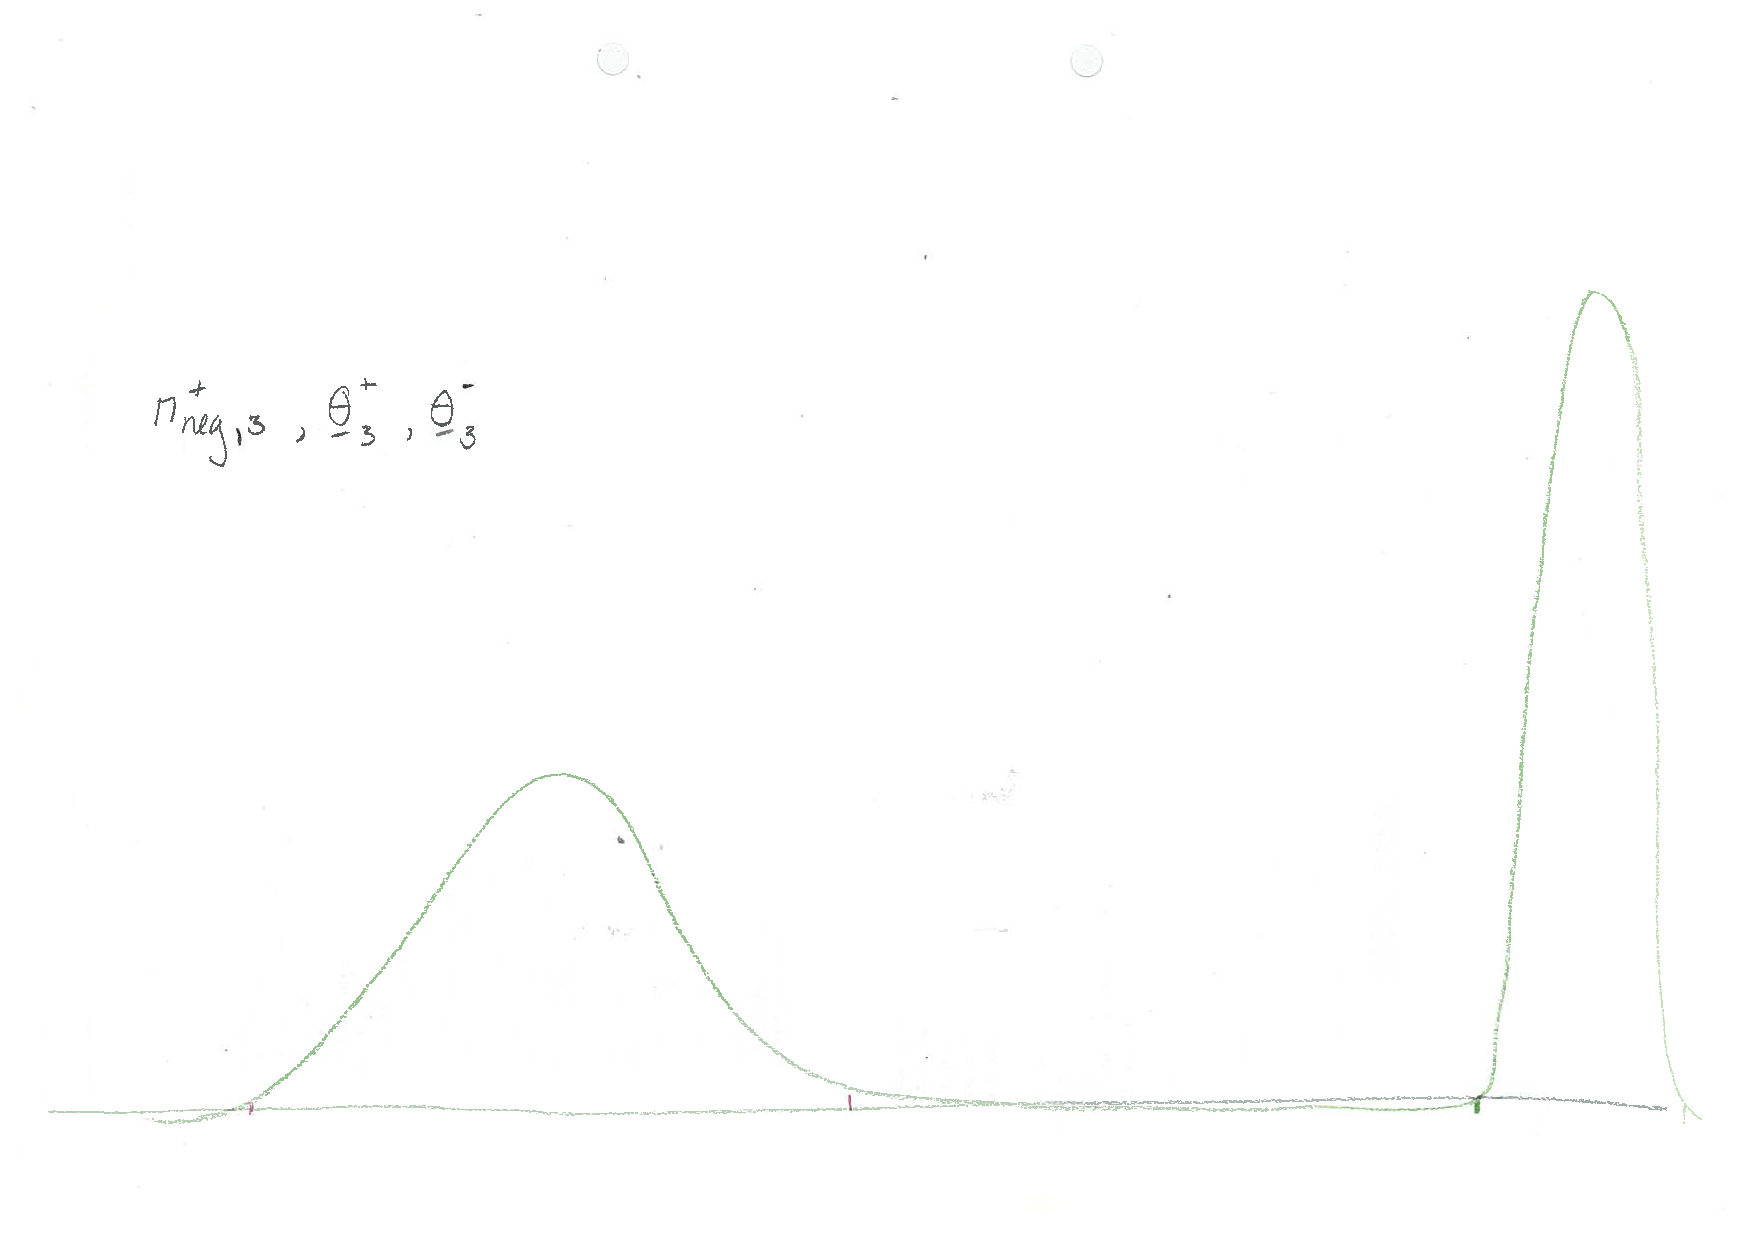
\includegraphics[height = 0.3\textheight]{/Volumes/kam025/Documents/Figures/Divergence_Manuscript/neg.pdf}
  \end{subfigure}
\end{figure}

The goal is to pick a divergence that is able to discriminate between $P_{p \_ bag}$ and $P_{n \_ bag}$ by measuring the dissimilarity to $P_{pos}$ and/or $P_{neg}$.
Let $\mathcal{X}_{pos > neg}$ be the region where $p_{pos}(x) > p_{neg}(x)$. 
Unless $p_{pos} = p_{neg}$ we have $\mathcal{X}_{pos > neg}$ nonempty, which gives $\mathcal{X}_{pos < neg}$ nonempty, whereas $\mathcal{X}_{pos = neg}$ might be empty or not. 

The Kullback-Leibler information (KL inf),
\begin{align}
  d_{KL}(p_{bag},p_{neg}) = \int_\mathcal{X} p_{bag}(x) \log \frac{p_{bag}(x)}{p_{neg}(x)} dx,
\end{align}
is a non-symmetric $f$-divergence.
The log ratio function gives a positive contribution whenever $p_{bag}>p_{neg}$, and a negative contribution for $p_{bag}<p_{neg}$, and zero contribution for $p_{bag} = p_{neg}$.
A large positive contribution for $p_{bag} >> p_{neg}$ and $p_{bag} >> 0$, which means that if $p_{bag}$ is outside the range of $p_{neg}$, the dissimilarity approaches infinity. 
This is a suitable property, because if $p_{bag}/p_{neg} \rightarrow \infty$, the probability the parameters of $p_{bag}$ are not sampled from the negative class. 
A simple straightforward measure is then
\begin{align}
  D(p_{bag},p_{neg}) = d_{KL} (p_{bag},p_{neg}),
\end{align}
and the ratio $d_{KL} (p_{bag},p_{pos})/d_{KL} (p_{bag},p_{neg})$ will give a classification rule.

%We will propose a divergence-based dissimilarity function where the two classes are integrated
%\begin{align}
%  D(p_{bag},p_{neg}|p_{pos}) = \int_{\mathcal{X}_{pos}} \frac{p_{pos}(x)}{p_{neg}(x)} p_{bag}(x) \log \frac{p_{bag}(x)}{p_{neg}(x)} dx
%\end{align}
%
%{\color{red} Have a look at this
%\begin{align}
%  \int_{\mathcal{X}_{neg}} \frac{p_{pos}(x)}{p_{neg}(x)} p_{bag}(x) \log \frac{p_{bag}(x)}{p_{neg}(x)} dx \leq \geq a \int_{\mathcal{X}_{neg}} p_{bag}(x) \log \frac{p_{bag}(x)}{p_{neg}(x)} dx
%\end{align}
%}

%\begin{align}
%  D^*(p_{bag},p_{neg}|p_{pos}) = \int_{\mathcal{X}_{pos}} \frac{p_{pos}(x)}{p_{neg}(x)} p_{bag}(x) \log \frac{p_{bag}(x)}{p_{neg}(x)} dx
%						+ \int_{\mathcal{X}_{neg}} \frac{p_{pos}(x)}{p_{neg}(x)} p_{bag}(x) \log \frac{p_{bag}(x)}{p_{neg}(x)} dx
%\end{align}

Because we also assume that $\pi_{pos} > \pi_{neg}$ it follows that $p_{p \_ bag} < p_{n \_ bag}, X \in \mathcal{X}_{neg}$ and therefore 
\begin{align}
  \int_{\mathcal{X}_{neg}} \frac{p_{pos}(x)}{p_{neg}(x)} p_{p\_bag}(x) \log \frac{p_{p\_bag}(x)}{p_{neg}(x)} dx < \int_{\mathcal{X}_{neg}} \frac{p_{pos}(x)}{p_{neg}(x)} p_{n \_ bag}(x) \log \frac{p_{n \_bag}(x)}{p_{neg}(x)} dx
\end{align}
which is an unwanted property, and therefore we use only $\mathcal{X}_{pos}$.

Like with KL inf, the log ratio function ensures large positive contributions for $p_{bag} >> p_{neg}$ when also $p_{bag} >> 0$. 
In addition, we require that $p_{pos} > p_{neg}$ for this contribution to be large. 
This is because if $p_{bag} >> p_{neg}$ but $p_{pos} < p_{neg}$ we have a bag whose pdf cannot be explained by the negative class, but neither by the positive class, and therefore is uninformative for classification. 
If $p_{pos} > p_{neg}$, or even $p_{pos} >> p_{neg}$, then $D \rightarrow \infty$.
How is this different from $d_{KL}(p_{bag},p_{pos})/d_{KL}(p_{bag},p_{neg})$?
If $p_{bag}/p_{pos} \rightarrow \infty$ and $p_{bag}/p_{neg} \rightarrow \infty$, then the ratio will be one. 

Why not use bag-to-bag?

\begin{align}
  \frac{p_{bag,b}}{p_{bag,b'}} \rightarrow \infty
\end{align}


